%% BioMed_Central_Tex_Template_v1.06

%%% additional documentclass options:
%  [doublespacing]
%  [linenumbers]   - put the line numbers on margins

%%% loading packages, author definitions

%\documentclass[twocolumn]{bmcart}% uncomment this for twocolumn layout and comment line below
\documentclass{configs/bmcart}

%%% Load packages
%\usepackage{amsthm,amsmath}
%\RequirePackage{natbib}
%\RequirePackage[authoryear]{natbib}% uncomment this for author-year bibliography
%\RequirePackage{hyperref}
%\usepackage[utf8]{inputenc} %unicode support
%\usepackage[applemac]{inputenc} %applemac support if unicode package fails
%\usepackage[latin1]{inputenc} %UNIX support if unicode package fails
\usepackage{booktabs}
\usepackage{graphicx}
\usepackage{url}
\usepackage[acronym]{glossaries}

%\makenoidxglossaries
\makeglossaries
\newacronym{roi}{ROI}{region of interest}
\newacronym{sfm}{SfM-MVS}{structure-from-motion multi-view stereo photogrammetry}
\newacronym{dom}{DOM}{digital orthophoto map}
\newacronym{dsm}{DSM}{digital surface model}
\newacronym{lidar}{LiDAR}{light detection and ranging}
\newacronym{ml}{ML}{machine learning}
\newacronym{dl}{DL}{deep learning}
\newacronym{pcd}{PCD}{point cloud data}
\newacronym{gis}{GIS}{geographic information system}
\newacronym{gcp}{GCPs}{ground control points}
\newacronym{mtp}{MTPs}{manual tie points}
\newacronym{mkl}{MKL}{math kernel library}
\newacronym{gui}{GUI}{graphical user interface}


%%%%%%%%%%%%%%%%%%%%%%%%%%%%%%%%%%%%%%%%%%%%%%%%%
%%                                             %%
%%  If you wish to display your graphics for   %%
%%  your own use using includegraphic or       %%
%%  includegraphics, then comment out the      %%
%%  following two lines of code.               %%
%%  NB: These line *must* be included when     %%
%%  submitting to BMC.                         %%
%%  All figure files must be submitted as      %%
%%  separate graphics through the BMC          %%
%%  submission process, not included in the    %%
%%  submitted article.                         %%
%%                                             %%
%%%%%%%%%%%%%%%%%%%%%%%%%%%%%%%%%%%%%%%%%%%%%%%%%

%\def\includegraphic{}
%\def\includegraphics{}


%%% Put your definitions there:
%\startlocaldefs
%\endlocaldefs


%%% Begin ...
\begin{document}

%%% Start of article front matter
\begin{frontmatter}

\begin{fmbox}
\dochead{Software}

%%%%%%%%%%%%%%%%%%%%%%%%%%%%%%%%%%%%%%%%%%%%%%
%%                                          %%
%% Enter the title of your article here     %%
%%                                          %%
%%%%%%%%%%%%%%%%%%%%%%%%%%%%%%%%%%%%%%%%%%%%%%

\title{EasyRIC: A post process tool for }


%%%%%%%%%%%%%%%%%%%%%%%%%%%%%%%%%%%%%%%%%%%%%%
%%                                          %%
%% Enter the authors here                   %%
%%                                          %%
%% Specify information, if available,       %%
%% in the form:                             %%
%%   <key>={<id1>,<id2>}                    %%
%%   <key>=                                 %%
%% Comment or delete the keys which are     %%
%% not used. Repeat \author command as much %%
%% as required.                             %%
%%                                          %%
%%%%%%%%%%%%%%%%%%%%%%%%%%%%%%%%%%%%%%%%%%%%%%

\author[
   addressref={aff1},
   %email={haozhou-wang@g.ecc.u-tokyo.ac.jp}
]{\inits{HW}\fnm{Haozhou} \snm{Wang}}
\author[
   addressref={aff1},
   corref={aff1}, 
   email={guowei@g.ecc.u-tokyo.ac.jp}
]{\inits{WG}\fnm{Wei} \snm{Guo}}

%%%%%%%%%%%%%%%%%%%%%%%%%%%%%%%%%%%%%%%%%%%%%%
%%                                          %%
%% Enter the authors' addresses here        %%
%%                                          %%
%% Repeat \address commands as much as      %%
%% required.                                %%
%%                                          %%
%%%%%%%%%%%%%%%%%%%%%%%%%%%%%%%%%%%%%%%%%%%%%%

\address[id=aff1]{
  \orgname{ International Field Phenomics Research Laboratory, Institute for Sustainable Agro-ecosystem Services, Graduate School of Agricultural and Life Science, The Univerisity of Tokyo}, 
  \postcode{188-0002} 
  \city{Tokyo}, 
  \cny{Japan}
}

%%%%%%%%%%%%%%%%%%%%%%%%%%%%%%%%%%%%%%%%%%%%%%
%%                                          %%
%% Enter short notes here                   %%
%%                                          %%
%% Short notes will be after addresses      %%
%% on first page.                           %%
%%                                          %%
%%%%%%%%%%%%%%%%%%%%%%%%%%%%%%%%%%%%%%%%%%%%%%

%\begin{artnotes}
%%\note{Sample of title note}     % note to the article
%\note[id=n1]{Equal contributor} % note, connected to %author
%\end{artnotes}

\end{fmbox}% comment this for two column layout

%%%%%%%%%%%%%%%%%%%%%%%%%%%%%%%%%%%%%%%%%%%%%%
%%                                          %%
%% The Abstract begins here                 %%
%%                                          %%
%% Please refer to the Instructions for     %%
%% authors on http://www.biomedcentral.com  %%
%% and include the section headings         %%
%% accordingly for your article type.       %%
%%                                          %%
%%%%%%%%%%%%%%%%%%%%%%%%%%%%%%%%%%%%%%%%%%%%%%

\begin{abstractbox}

\begin{abstract}
\parttitle{Background} 
Applying high-throughput phenotyping technologies in agriculture provides an advanced and efficient method for managing and breeding crops in practical applications. Compared with device-specified remote sensing technologies (laser scanning, \acrfull*{lidar}, etc.), \acrfull*{sfm}, applicable to price friendly RGB digital cameras, has been widely spread use around the world, and many commercial and open-source software are available to implement this task. However, producing good quality of its products, such as \acrfull*{dom}, \acrfull*{dsm}, and point clouds, is quite computation intensive and hard to meet the same precision of original photos. Hence, linking low computation time produced low quality \acrshort*{sfm} products back to original digital images has significant potential to improve the efficiency and precision for data processing, but to the best of our knowledge, no easy-to-use open source tool is available for this object.

\parttitle{Results}
In this study, a pure python package called EasyRIC (easy reconstruction image converter) was developed to link original photos to \acrshort*{sfm} products. The Lotus (\textit{Nelumbo nucifera}) breeding field were used as a show case to demonstrate the following functions: 1) Clipping the \acrfull*{roi} from point clouds and compare them throught time series. 2) Clipping the \acrshort*{roi} from \acrshort*{sfm} products to raw images. 3) Generate bunch of training data in raw images from a few manual marked \acrshort*{roi}.

\parttitle{Conclusions}
This python package shows the great potential to integrate the high-quality original images with  \acrshort*{sfm} produced products. The quick produced low quality products are also acceptable which saved plenty computation time. Also this tool can be used to generate bunch of training data for machine learning with a few manual operation.

\end{abstract}

%%%%%%%%%%%%%%%%%%%%%%%%%%%%%%%%%%%%%%%%%%%%%%
%%                                          %%
%% The keywords begin here                  %%
%%                                          %%
%% Put each keyword in separate \kwd{}.     %%
%%                                          %%
%%%%%%%%%%%%%%%%%%%%%%%%%%%%%%%%%%%%%%%%%%%%%%

\begin{keyword}
\kwd{3D reconstruction}
\kwd{Orthomosaic}
\kwd{Training data generation}
\kwd{Phenotyping}
\kwd{Open source}
\kwd{Pix4D}
\end{keyword}

\end{abstractbox}
%
%\end{fmbox}% uncomment this for twcolumn layout

\end{frontmatter}

%%%%%%%%%%%%%%%%%%%%%%%%%%%%%%%%%%%%%%%%%%%%%%
%%                                          %%
%% The Main Body begins here                %%
%%                                          %%
%% Please refer to the instructions for     %%
%% authors on:                              %%
%% http://www.biomedcentral.com/info/authors%%
%% and include the section headings         %%
%% accordingly for your article type.       %%
%%                                          %%
%% See the Results and Discussion section   %%
%% for details on how to create sub-sections%%
%%                                          %%
%% use \cite{...} to cite references        %%
%%  \cite{koon} and                         %%
%%  \cite{oreg,khar,zvai,xjon,schn,pond}    %%
%%  \nocite{smith,marg,hunn,advi,koha,mouse}%%
%%                                          %%
%%%%%%%%%%%%%%%%%%%%%%%%%%%%%%%%%%%%%%%%%%%%%%

\section*{Background}
Para1: Agricultural crisis -> demand for high-throughput phenotyping

Para2: Common high-throughput phenotyping technologies -> why RGB SfM

Para3: SfM background, \textbf{algorithm}, and software (computation intensive drawbacks, need low quality to save time)

Para4: Data processing (the difficulties to of use the result of SfM, e.g. 1) low quality of DOM make canopy cover, organ detection. -> link to raw image; 2) 3D analysis not easy (require large RAM and good computation to processing point cloud, and the quality of point cloud couldn't too large -> 3D to 2d, 3D clipping, there is no common tool to make this transfer easy)

%Pix4D OpenSFM, FieldReconst (http://cse.naro.affrc.go.jp/rsugiura/FieldReconst/) introduction

Para5: 4D time series analysis demand and point cloud clipping

Para6: Training Data crisis

Para7: Objectives

\section*{Implementation}

This study implemented a open-source python \cite{guido_python_2020} package called EasyRIC (easy reconstruction image converter) to cropping \acrshort*{sfm} software (e.g. Pix4Dmapper, Metashape, etc.) produced products based on \acrfull*{roi} and linking them on original images. Though the source codes were cross-platform due to the characteristic of python language, they were programmed and tested under Windows 10 64-bit platform and Intel CPU with \acrfull*{mkl} support. For the package performance reliability, the 8GB of RAM and CPU with at 3.0 GHz are recommended. The requirements to use this packages requires: the Python >= 3.7, numpy >= 1.18.1, scikit-image >= 0.16.2, opencv-python >= 3.4.2.16, pyproj==2.6.1.post1, pyparsing>=2.0.1 are required, and following pure python packages were included in source code without installation: Pyshp, Send2Trash, ezdxf, and plyfile. The user manual and source code can be accessed via: https://github.com/HowcanoeWang/EasyRIC and the License is GPL-3.0 which is free to use for any purpose, forever.

The general workflow of this tool was shown in Figure \ref{fig:workflow}. There were three main parts of this workflow, including two input data preparations: 3D reconstruction outputs (Figure \ref{fig:workflow}.a) and corresponding \acrfull*{roi} by other tools (Figure \ref{fig:workflow}.b); and EasyRIC converting tool core functions (Figure \ref{fig:workflow}.c). Each part had tight correspondence with 3D reconstruction workflow, and was split into (1) SfM stage, (2) MVS stage, and (3) GIS stage respectively. 

The first SfM stage (Figure \ref{fig:workflow}.c-1) provides the experimental function that convert the \acrfull*{roi} on one raw images (2D) to the other raw images (2D) just after SfM stages ("2D to 2D") in \acrlong*{sfm} software without further time-consuming MVS densification and GIS outputs steps. It saves a plenty of time in data processing, however, our case study pre-experiment result (Appendix A) showed this experimental stage still needs great improvements to make the accuracy acceptable.

The second MVS stage (Figure \ref{fig:workflow}.c-2) transforms the \acrfull*{roi} on point cloud data (3D) to the related raw images (2D) after MVS densification in \acrlong*{sfm} software ("3D to 2D"). 

The third GIS stage (Figure \ref{fig:workflow}.c-3) transforms the \acrfull*{roi} on \acrfull*{gis} products to related raw images (2D). Commonly, the ROI is marked manually by GIS software on \acrfull*{dom}. The height information is provided by \acrfull*{dsm}. Compared with 3D information extracted directly on point clouds, this geometry information is combined by XY axis from DOM and Z axis from DSM, named 2.5D to distinguish with point cloud 3D. This stage is also specified as "2.5D to 2D".

\subsection*{Input data preparation}

\subsubsection*{Image collection}
pass

\subsubsection*{3D reconstruction by SfM-MVS}
%The definition of each camera external parameters and 2D \& 3D coordinates

%including lens distortion correction (default FC550\_DJI camera model), automatic feature tie-points matching, manual \acrfull*{gcp} marking via ??? GPS device (Figure \ref{fig:map}.c), building densified point clouds, and exporting both \acrshort*{dom} and \acrshort*{dsm}.

%build the sparse tie-point cloud, and also produce the geometry relationship among each raw images. The geometry relationship reflects in the output files, including distortion corrected images

the internal and external camera parameters, and pmatrix referred to camera matrix

% miller_estimate_2015 里面有SfM-MVS的所有操作步骤

based on the optional ground define step via \acrfull*{gcp} or \acrfull*{mtp}

\subsubsection*{Region of Interest (ROI) making}
(1) for making 2D pixel coordinates on raw or undistorted images, common photo processing software can be used, e.g. open-source GIMP or commercial Photoshop. (2) for making 3D coordinates in point cloud (or 3D geographic coordinates if ground defined), common 3D processing software can be used, e.g. CloudCompare or MeshLab. (3) for making 2D geographic polygon on DOM and DSM, common \acrfull*{gis} processing software including QGIS (open source) or ArcMap (commercial) can be used to produce required shapefiles.

"2D to 2D": For those predefined ground plots, the image analyzing software (e.g. Photoshop, GIMP, etc.) was used to mark 2D pixel coordinates of \acrshort*{roi} on one original images, and calculate the 2D pixel coordinates of this \acrshort*{roi} on other original images.

"3D to 2D": For both predefined and non-predefined ground plots, the \acrfull*{pcd} and point cloud analyzing software (e.g. CloudCompare) were used to obtain 3D \acrshort*{roi} directly, and the same reverse calculation as previous class was applied afterwards. The details of this method, algorithms and testing experimental plots were given below.

...(dxm2raw, extract height from DSM and obtain 3D geographic coordinates of pcd2raw) and clipping DOM and DSM by ROI (dxm2part).

"2.5D to 2D": For those predefined ground plots, the DOM and \acrfull*{gis} software were used to produce 2D \acrshort*{roi} polygon shapefile (*.shp), and the DSM was used to obtain the height (Z axis) values in order to get the 3D coordinates of \acrshort*{roi}. Then the reverse calculation was applied to calculate the 2D pixel coordinates of this \acrshort*{roi} on given original images based on the joint rotation-translation matrix (also called camera matrix or pmatrix) produced by \acrshort*{sfm} software.

\subsection*{Package Algorithms}

It is a python package without any \acrfull*{gui}, all the performance a based on API, please refer to the following link https://www.to.be.continued.org. Instead of introducing how the package is used, this section demonstrate the algorithm for calculation

\subsubsection*{Input and output files}
% Input: Shp, DXM_header, PCD, 3D dxf

\subsubsection*{How to 2D to 2D}
pass

\subsubsection*{How to 2.5D to 2D}
pass

\subsubsection*{How to 3D to 2D}
pass

\subsection*{Case Study: Lotus Ponds}

\subsubsection*{Field data and image collection}
To obtain the materials for package developing and testing, a lotus (\textit{Nelumbo nucifera}) experimental plot in Nishi-Tokyo, Tokyo, Japan was used as a case study (Figure \ref{fig:map}.a). The total 112 different varieties of lotus were sown in squire cultivation ponds on the ???, 2017 (Figure \ref{fig:map}.b). The ordinary local management practices were used to managed all trails.

The DJI FC550 drone (VC Technology, UK) was used to acquire images, the flight height is 30 m and the flight speed is ??? m/s. The flight route was designed by ??? software and the heading overlap and side overlap were ??? \% and ??? \% respectively. The Pix4Dmapper Pro software (Pix4D, Lausanne, Switzerland) was used to obtain the \acrshort*{sfm} products. The parameters for all \acrshort*{sfm} steps in the software were used as default, and the \acrfull*{gcp} were marked by ??? GPS device (Figure \ref{fig:map}.c). The device for 3D reconstruction processing includes Intel Xeon E5-2690 v4 @2.60GHz CPU; 128GB RAM; two NVIDIA GeForce GTX1080Ti (Driver: 26.21.14.3186) GPUs; and Windows 10 Pro, 64-bit operating system. The details of digital data collected and produced were shown in Table \ref{tab:diginfo}.

\subsection*{Accuracy assessment and evaluation}
%IoU calculation and \cite{tresch_easy_2019}

\subsubsection*{Intersection of union (IoU)}

\subsubsection*{Time-series traits evaluation}
% calculation of coverage

% calculation of height



\section*{Results}

\subsection*{Use case 1: Point cloud segmentation}
Compare \acrshort*{roi} by time series

In this part, both raw photo? DOM? and point clouds should be displayed? Clipping point clouds may requires Open3D packages, which can not guarantee easy to be packed up.

\subsection*{Use case 2: plot segmentation}

Find \acrshort*{roi} in \acrshort*{sfm} products on the raw images

text \cite{ma_calculation_2019, guo_illumination_2013}
should including from DOM(DSM) coordinates (GIS or pixel) and point clouds (3D) coordinates to raw images.

\subsection*{Use case 3: Efficient annotation of training data for ML/DL}
3D/2.5D small region -> 2D->Raw small region, selecting strategy for efficient annotation of training data for ML/DL.

\section*{Discussion}

%\subsection*{Future prospects}
API for most \acrshort*{sfm} software packages

2D Photo to 2D photo without SfM products

Link between Aerial and Terrestrial photos.

\section*{Conclusions}
Text

\section*{Availability and requirements}
\begin{itemize}
  \item \textbf{Project name:} EasyRIC
  \item \textbf{Project home page:} https://github.com/HowcanoeWang/EasyRIC
  \item \textbf{Operating system(s):} Using the source codes as Python package is platform independent, also providing executable software package for windows (windows 10 and 64-bit is tested and recommended).
  \item \textbf{Programming language: } Python
  \item \textbf{Other requirements:} For using source code as package: Python 3.7 or higher, numpy 1.18.1 or higher, scikit-image 0.16.2 or higher; For using executable software packages on Windows, 64-bit windows is required, and Intel CPU (with mkl support) is recommended.
  \item \textbf{License:} GPL-3.0
  \item \textbf{Any restrictions to use by non-academics:} Free to use for any purpose, forever.
\end{itemize}

%\paragraph*{Sub-sub-sub heading for section}
%Text for this sub-sub-sub-heading.

%%%%%%%%%%%%%%%%%%%%%%%%%%%%%%%%%%%%%%%%%%%%%%
%%                                          %%
%% Backmatter begins here                   %%
%%                                          %%
%%%%%%%%%%%%%%%%%%%%%%%%%%%%%%%%%%%%%%%%%%%%%%

\begin{backmatter}

%\section*{Abbreviations}
\renewcommand*{\glsgroupskip}{}
\printglossary[type=\acronymtype, title=Abbreviations]

\section*{Competing interests}
  The authors declare that they have no competing interests.

\section*{Author's contributions}
  Text for this section \ldots

\section*{Acknowledgements}
  Text for this section \ldots

%%%%%%%%%%%%%%%%%%%%%%%%%%%%%%%%%%%%%%%%%%%%%%%%%%%%%%%%%%%%%
%%                  The Bibliography                       %%
%%                                                         %%
%%  Bmc_mathpys.bst  will be used to                       %%
%%  create a .BBL file for submission.                     %%
%%  After submission of the .TEX file,                     %%
%%  you will be prompted to submit your .BBL file.         %%
%%                                                         %%
%%                                                         %%
%%  Note that the displayed Bibliography will not          %%
%%  necessarily be rendered by Latex exactly as specified  %%
%%  in the online Instructions for Authors.                %%
%%                                                         %%
%%%%%%%%%%%%%%%%%%%%%%%%%%%%%%%%%%%%%%%%%%%%%%%%%%%%%%%%%%%%%

\bibliographystyle{configs/vancouver} % Style BST file (bmc-mathphys, vancouver, spbasic).
\bibliography{myzotero}

%%%%%%%%%%%%%%%%%%%%%%%%%%%%%%%%%%%
%%                               %%
%% Figures                       %%
%%                               %%
%% NB: this is for captions and  %%
%% Titles. All graphics must be  %%
%% submitted separately and NOT  %%
%% included in the Tex document  %%
%%                               %%
%%%%%%%%%%%%%%%%%%%%%%%%%%%%%%%%%%%

%%
%% Do not use \listoffigures as most will included as separate files

\section*{Figures}

\begin{figure}[!h]
  %\centering
  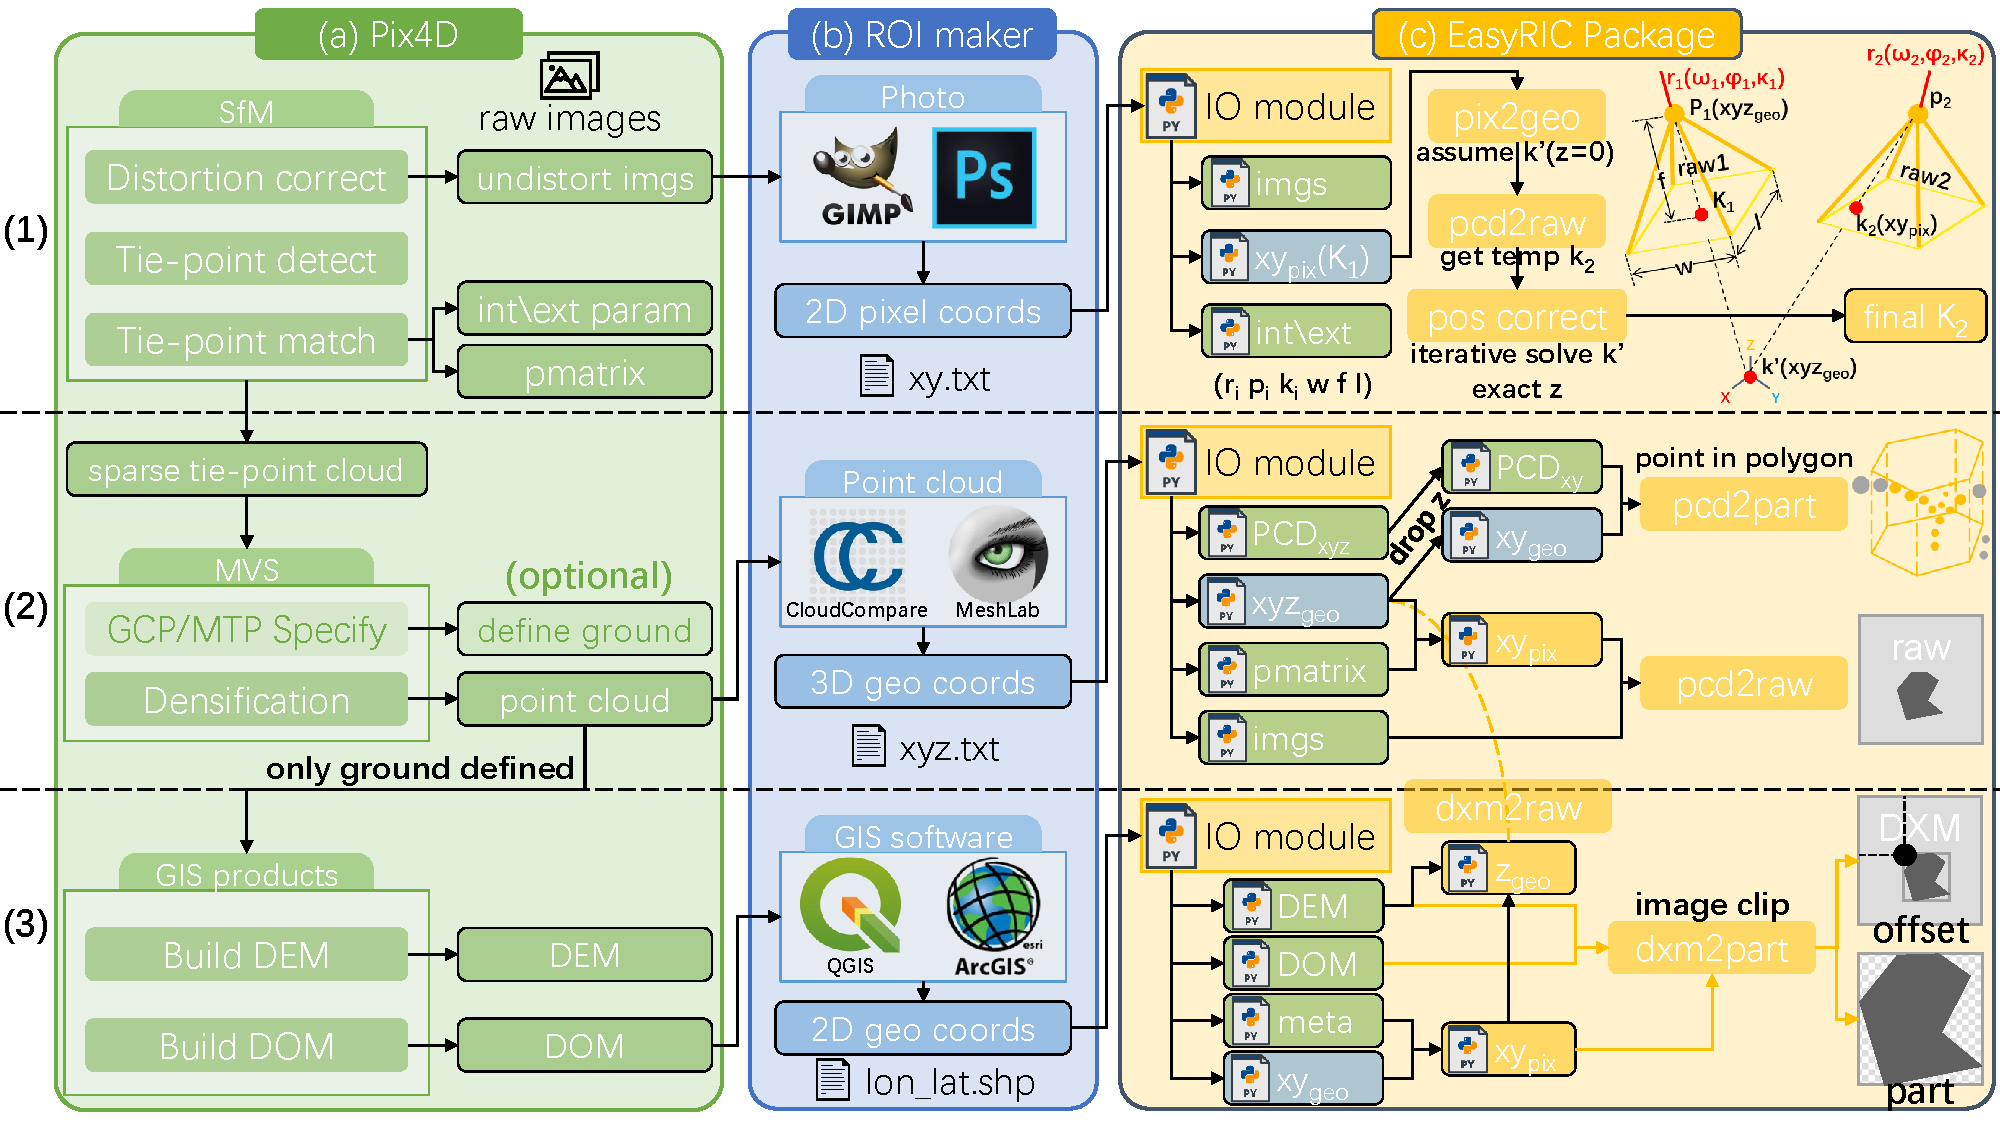
\includegraphics[width=0.95\linewidth]{figures/workflow.pdf}
  \caption{The workflow of proposed method. (\textbf{a}) The processing pipeline and output of 3D reconstruction (use Pix4Dmapper as example). This step can be separated into 3 parts: (1) the structure from motion (SfM) part which build the sparse tie-point cloud. (2) the multi-view stereo (MVS) photogrammetry part which densify previous sparse tie-point cloud and make geographic corrections. (3) For those defined ground plots, export \acrfull*{dom} and \acrfull*{dsm}. (\textbf{b}) The \acrfull*{roi} maker pipeline via commercial or open source tools. (\textbf{c}) The processing pipeline for EasyRIC package, (1) "2D to 2D" part (ROI from image 1 to image 2). $r_i$ represented camera rotation of image $i$; $p_i$, represented camera position of image $i$; $k_i$ represented 2D pixel coordinates on image $i$; $w$ was sensor width (mm); $f$ was sensor focal length, and $l$ was sensor length (mm). (2) "3D to 2D" part (ROI from point cloud data to raw images). (3) "2.5D to 2D part" (ROI from geographic shapefile to raw images)}
  \label{fig:workflow}
\end{figure}

\begin{figure}[!h]
  %\centering
  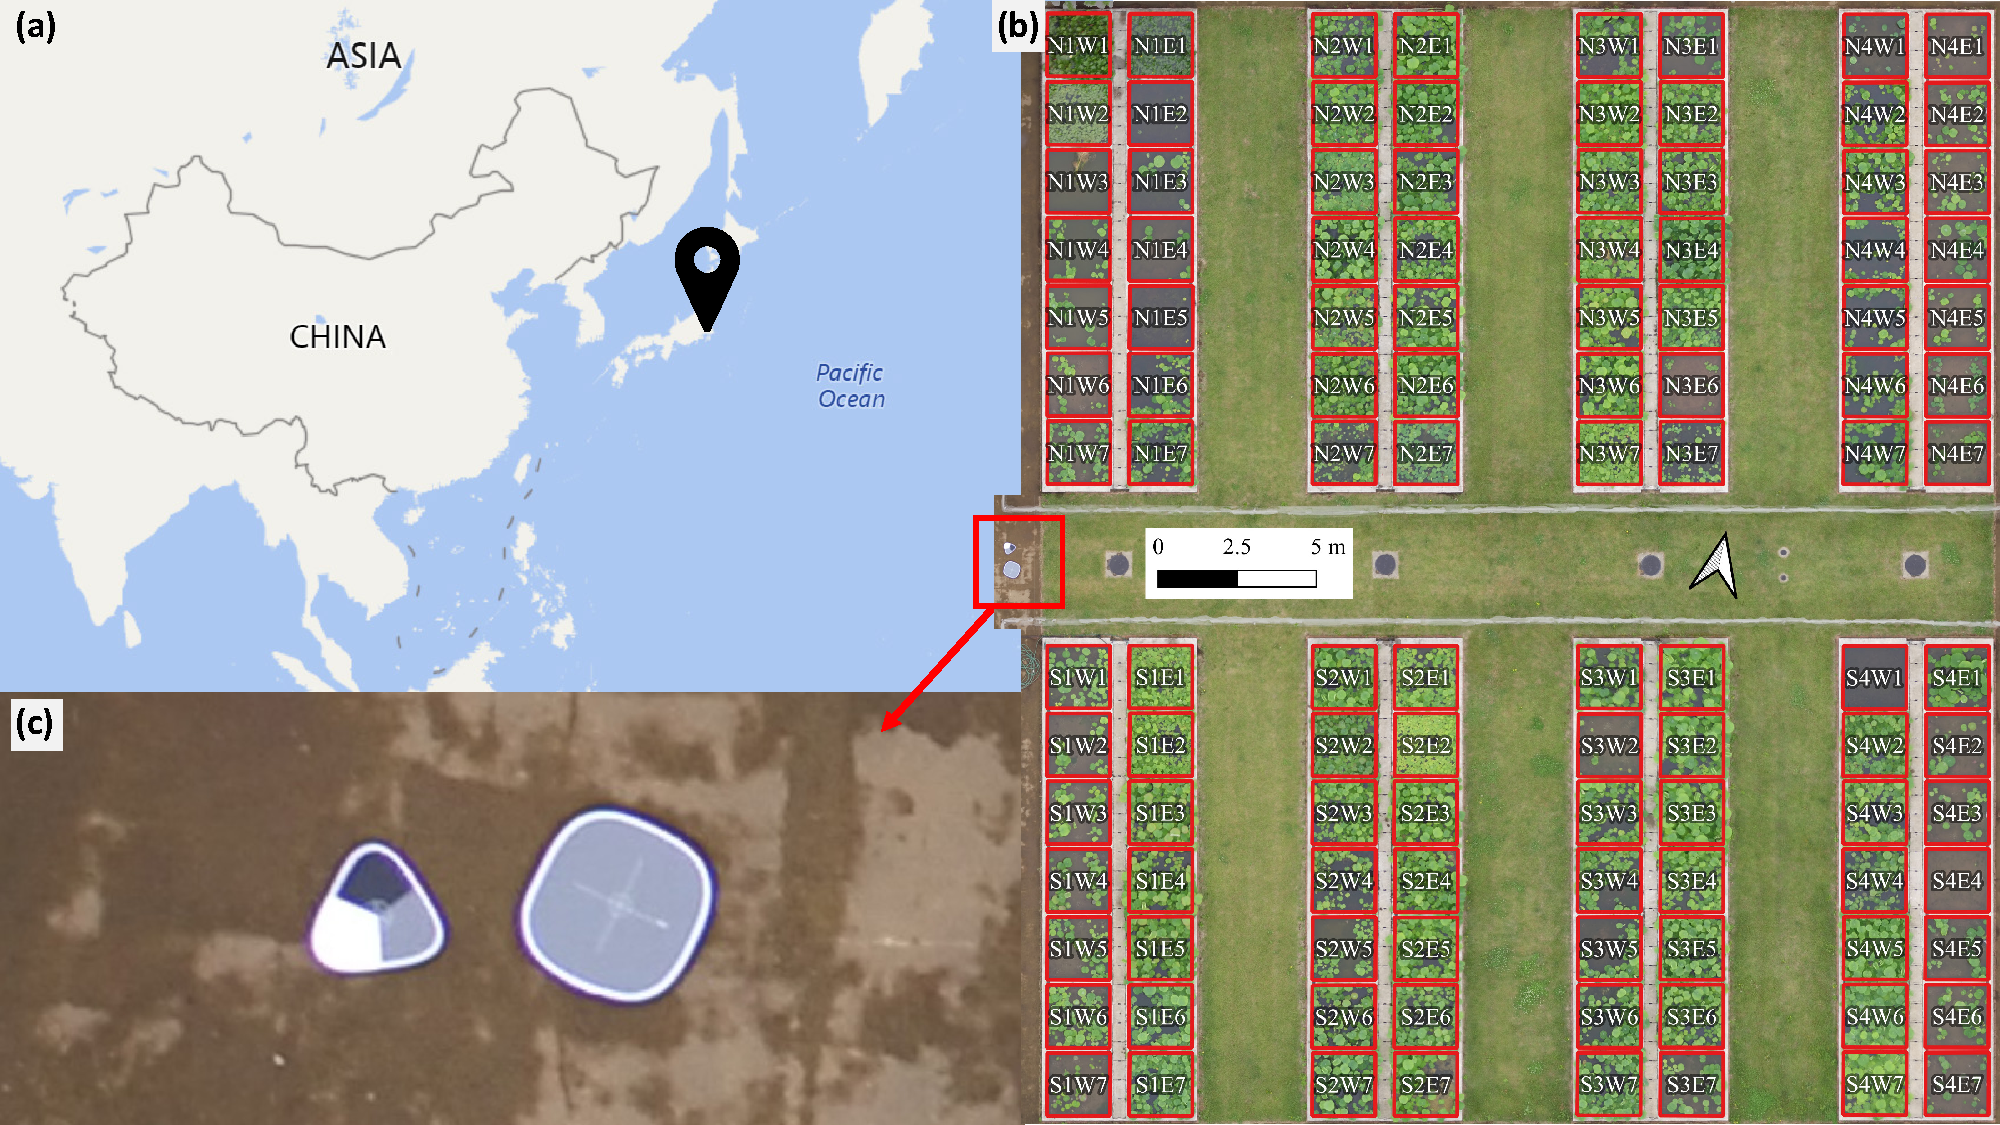
\includegraphics[width=0.95\linewidth]{figures/map.pdf}
  \caption{The experimental lotus plot condition. (\textbf{a}) the experimental plot locates in Nishi-Tokyo, Tokyo, Japan; (\textbf{b}) The labels of cultivation ponds, the orthomosaic showed here was collected on the May 5, 2017. The labels and boundaries of ponds were made by QGIS software and saved to shapefile (\*.shp) for later usage; (\textbf{c}) shows the device used for obtaining geographic position and functioning as ground control point to linking different flight time series together}
  \label{fig:map}
\end{figure}

\begin{figure}[!h]
  %\centering
  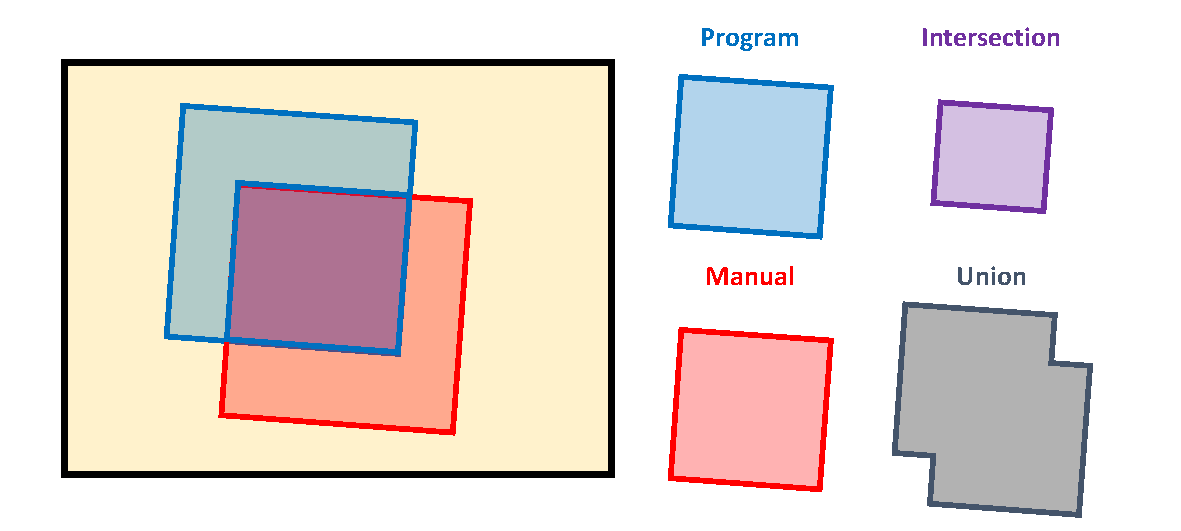
\includegraphics[width=0.95\linewidth]{figures/iou.pdf}
  \caption{The diagram of \acrfull*{iou} calculation. The red polygon is manual marking by LabelMe, the blue polygon is EasyRIC program calculated \acrfull*{roi} on raw images. The purple polygon is the intersection of two results while the gray polygon is the union of them. The IoU equals to the intersection divide by the union.}
  \label{fig:iou}
\end{figure}

\begin{figure}[!h]
  %\centering
  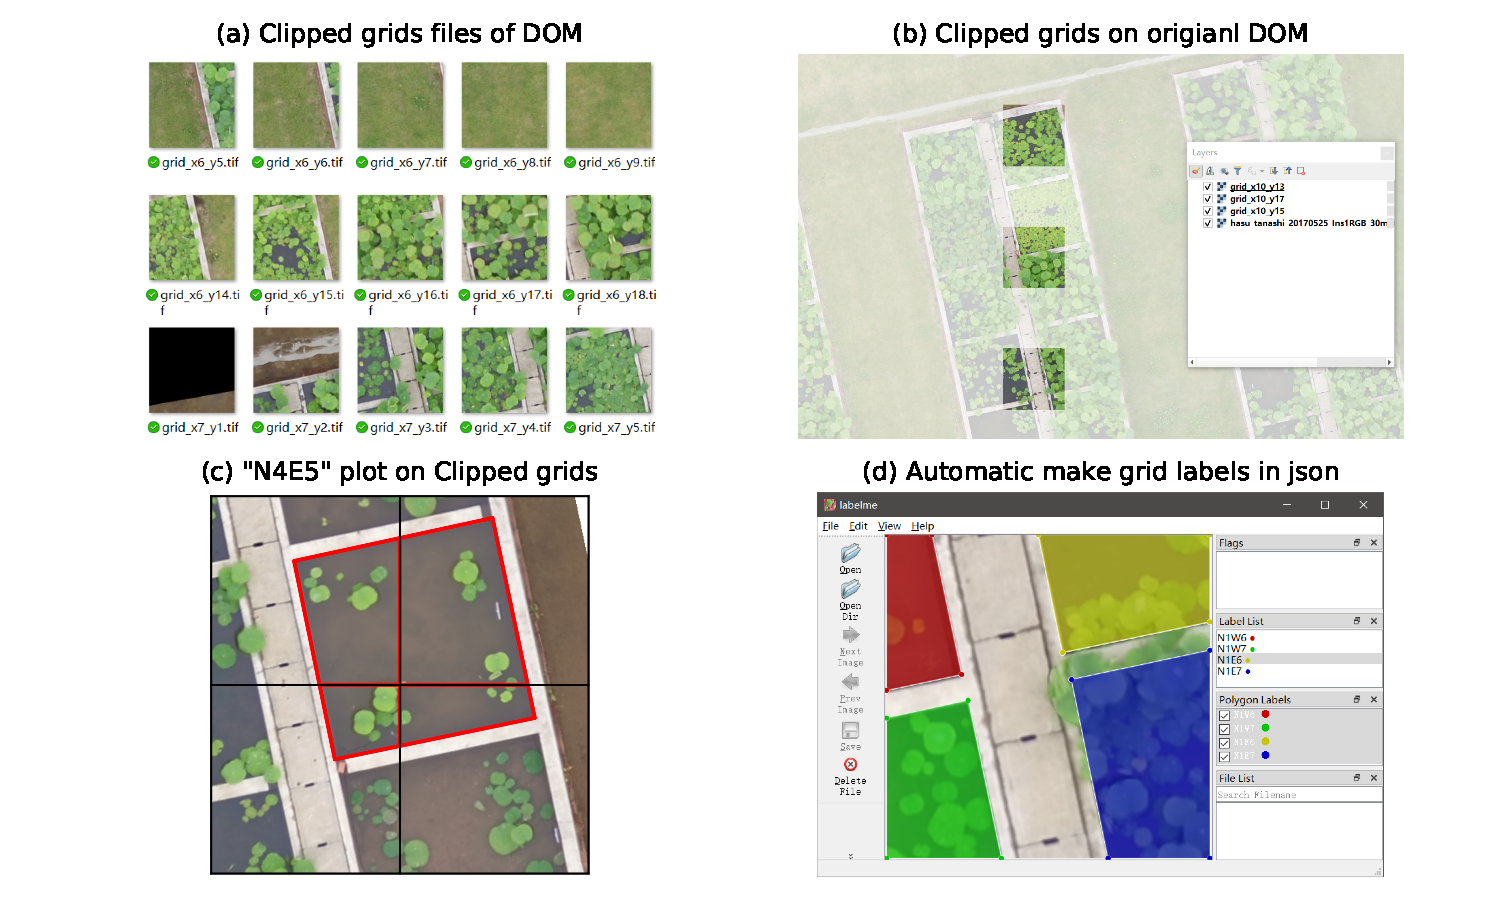
\includegraphics[width=0.95\linewidth]{figures/dom2grids.pdf}
  \caption{tbc}
  \label{fig:dom2girds}
\end{figure}

\begin{figure}[!h]
  %\centering
  \includegraphics[width=0.95\linewidth]{figures/roi2dxm.pdf}
  \caption{tbc}
  \label{fig:roi2dxm}
\end{figure}

\begin{figure}[!h]
  %\centering
  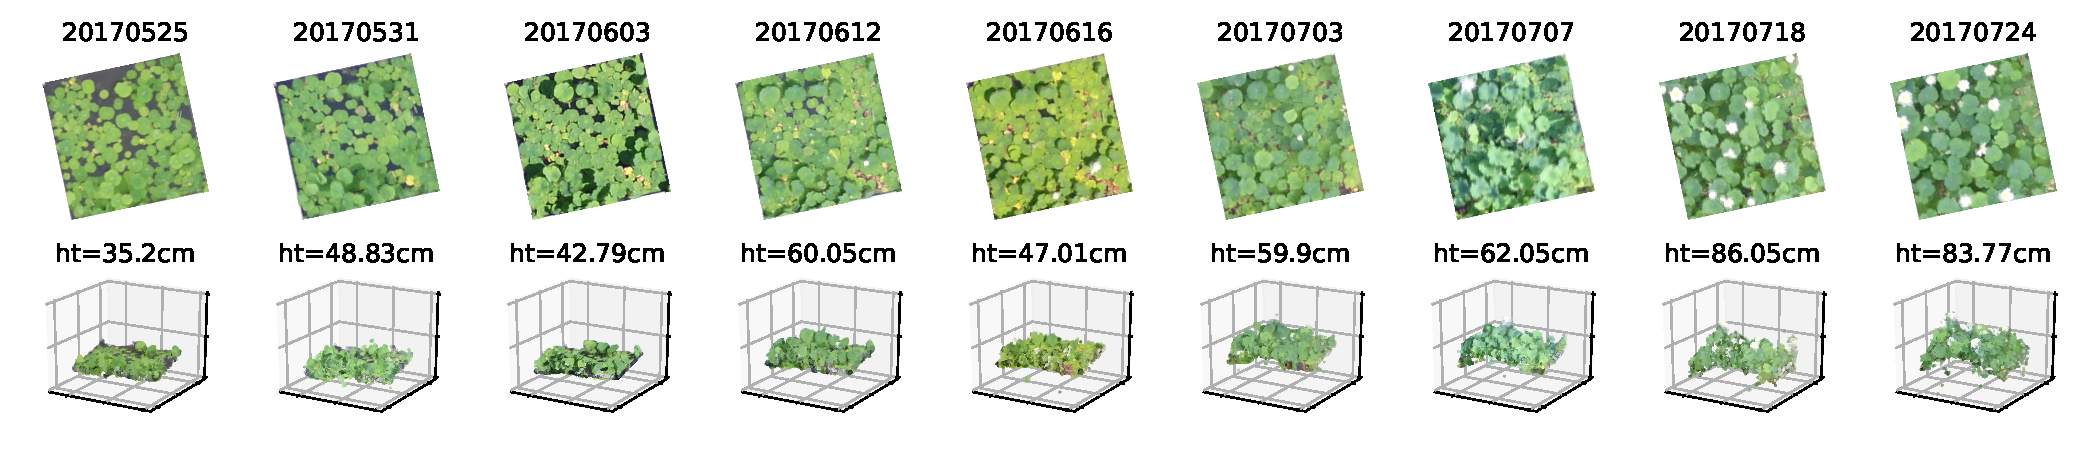
\includegraphics[width=0.95\linewidth]{figures/time_series.pdf}
  \caption{tbc}
  \label{fig:time}
\end{figure}


\begin{figure}[!h]
  %\centering
  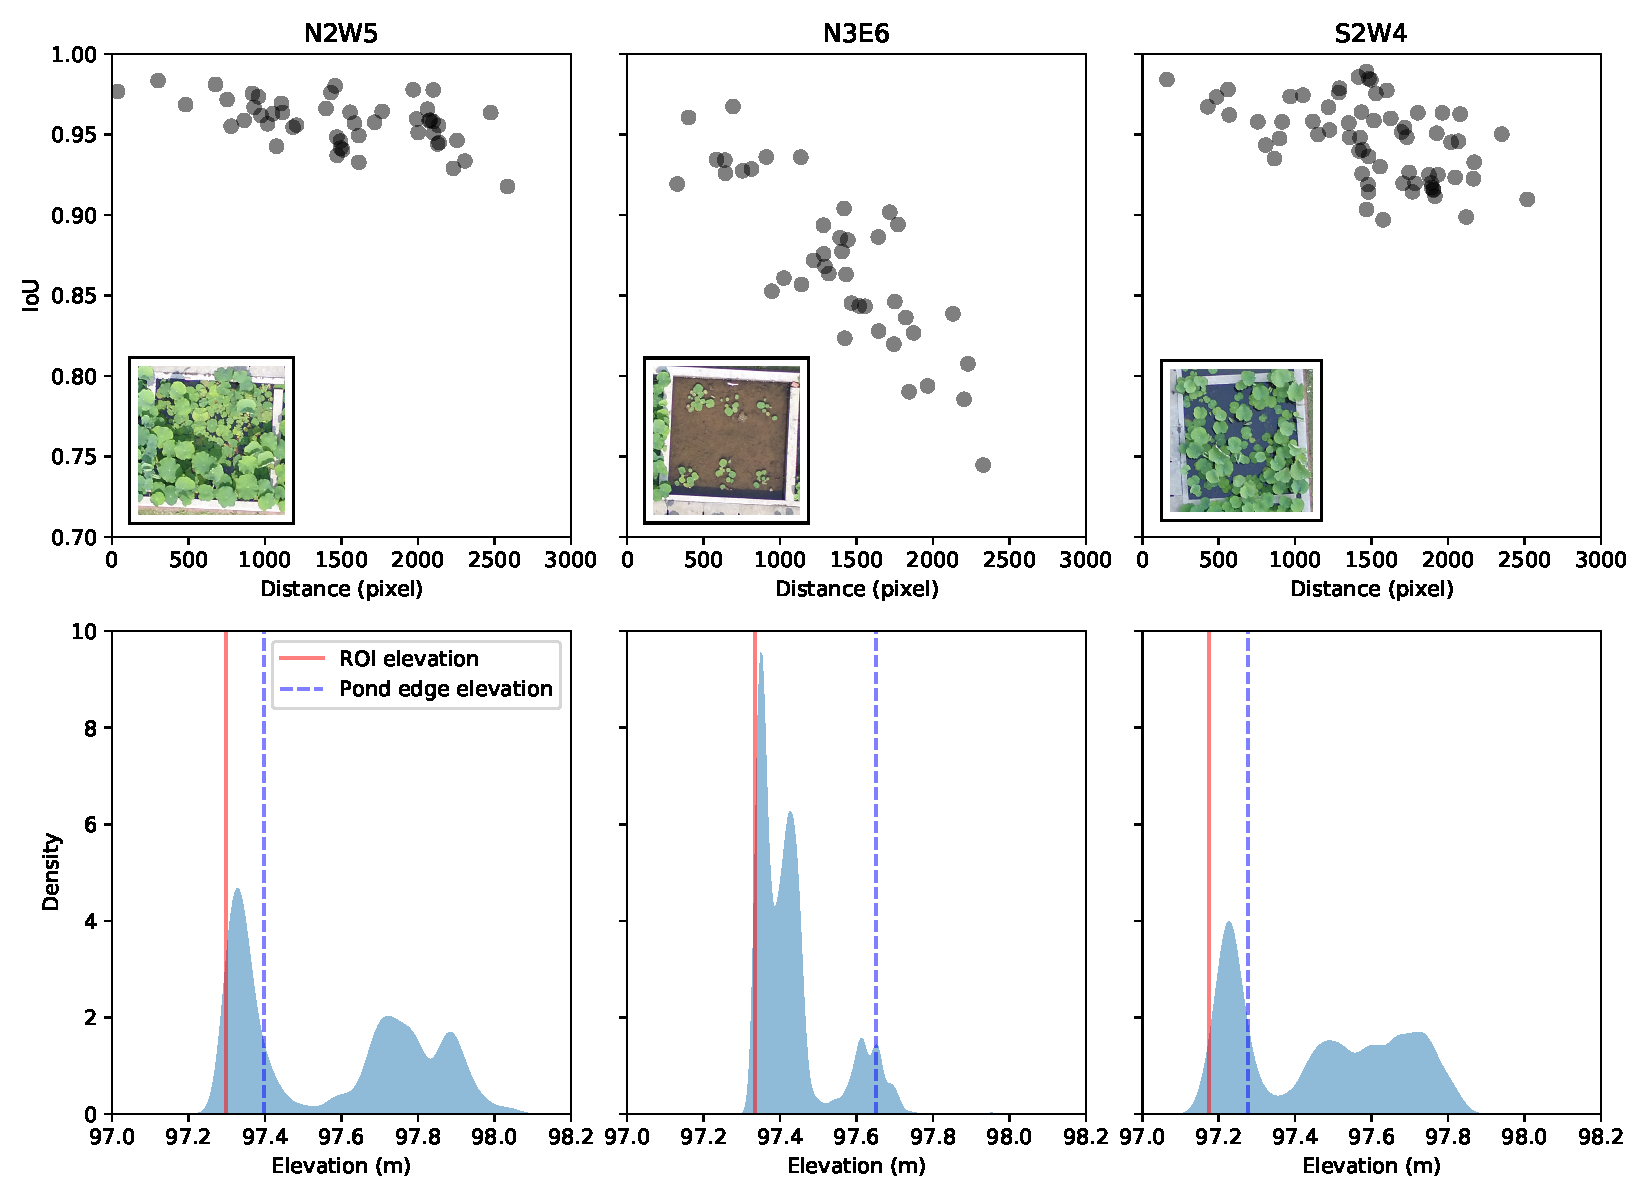
\includegraphics[width=0.95\linewidth]{figures/dist.pdf}
  \caption{tbc}
  \label{fig:dist}
\end{figure}

\begin{figure}[!h]
  %\centering
  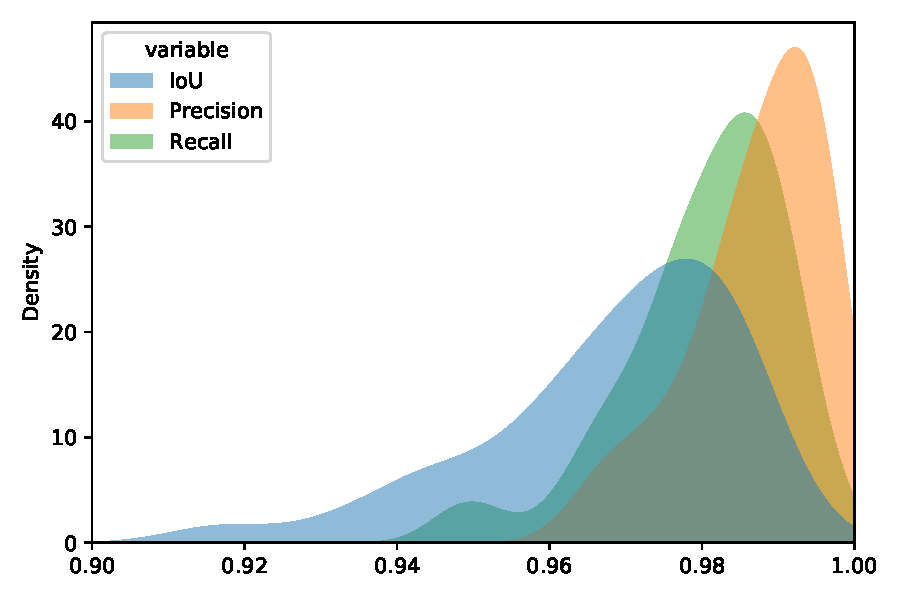
\includegraphics[width=0.95\linewidth]{figures/iou_all.pdf}
  \caption{tbc}
  \label{fig:iou_all}
\end{figure}

%%%%%%%%%%%%%%%%%%%%%%%%%%%%%%%%%%%
%%                               %%
%% Tables                        %%
%%                               %%
%%%%%%%%%%%%%%%%%%%%%%%%%%%%%%%%%%%

%% Use of \listoftables is discouraged.
%%
\section*{Tables}

\begin{table}[!h]
  \caption{Trail field and image collection information}
  \centering
  %% \tablesize{} %% You can specify the fontsize here, e.g., \tablesize{\footnotesize}. If commented out \small will be used.
  \resizebox{\textwidth}{!}{
  \begin{tabular}{ccccccc}
    \toprule
    \textbf{Flight date}	& \textbf{No. of raw images}	& \textbf{Size of raw images} & \textbf{Size of DOM} & \textbf{Size of DSM} & \textbf{Size of PCD}  & \textbf{Processing time} \\ 
    (yyyymmdd)&     & (GB) & (MB) & (MB) & (MB) & (min)\\
    \midrule
    20170525  & 266	& 1.64 & 38.5 & 34.6 & 89.2 & 39.7 \\
    20170531	& 151 & 0.94 & 40.4 & 37.6 & 60.0 & 47.3 \\
    20170603	& 141 & 0.87 & 46.5 & 34.1 & 60.3 & 18.8 \\
    20170612	& 285 & 1.74 & 38.1 & 32.9 & 93.8 & 101.5\\
    20170616	& 136 & 0.84 & 39.1 & 33.4 & 60.1 & 11.1 \\
    20170703	& 138 & 0.88 & 36.3 & 33.2 & 58.5 & 11.0 \\
    20170707	& 132 & 0.82 & 40.7 & 32.4 & 57.1 & 10.0 \\
    20170711	& 138 & 0.86 & 41.8 & 33.4 & 57.8 & 14.4 \\
    20170718	& 135 & 0.84 & 38.5 & 35.4 & 56.9 & 10.1 \\
    20170724	& 142 & 0.90 & 34.5 & 32.9 & 59.2 & 10.3 \\
    \bottomrule
  \end{tabular}
  }
  \label{tab:diginfo}
\end{table}

%%%%%%%%%%%%%%%%%%%%%%%%%%%%%%%%%%%
%%                               %%
%% Additional Files              %%
%%                               %%
%%%%%%%%%%%%%%%%%%%%%%%%%%%%%%%%%%%

\section*{Additional Files}
  \subsection*{Additional file 1 --- Sample additional file title}
  \begin{figure}[!h]
    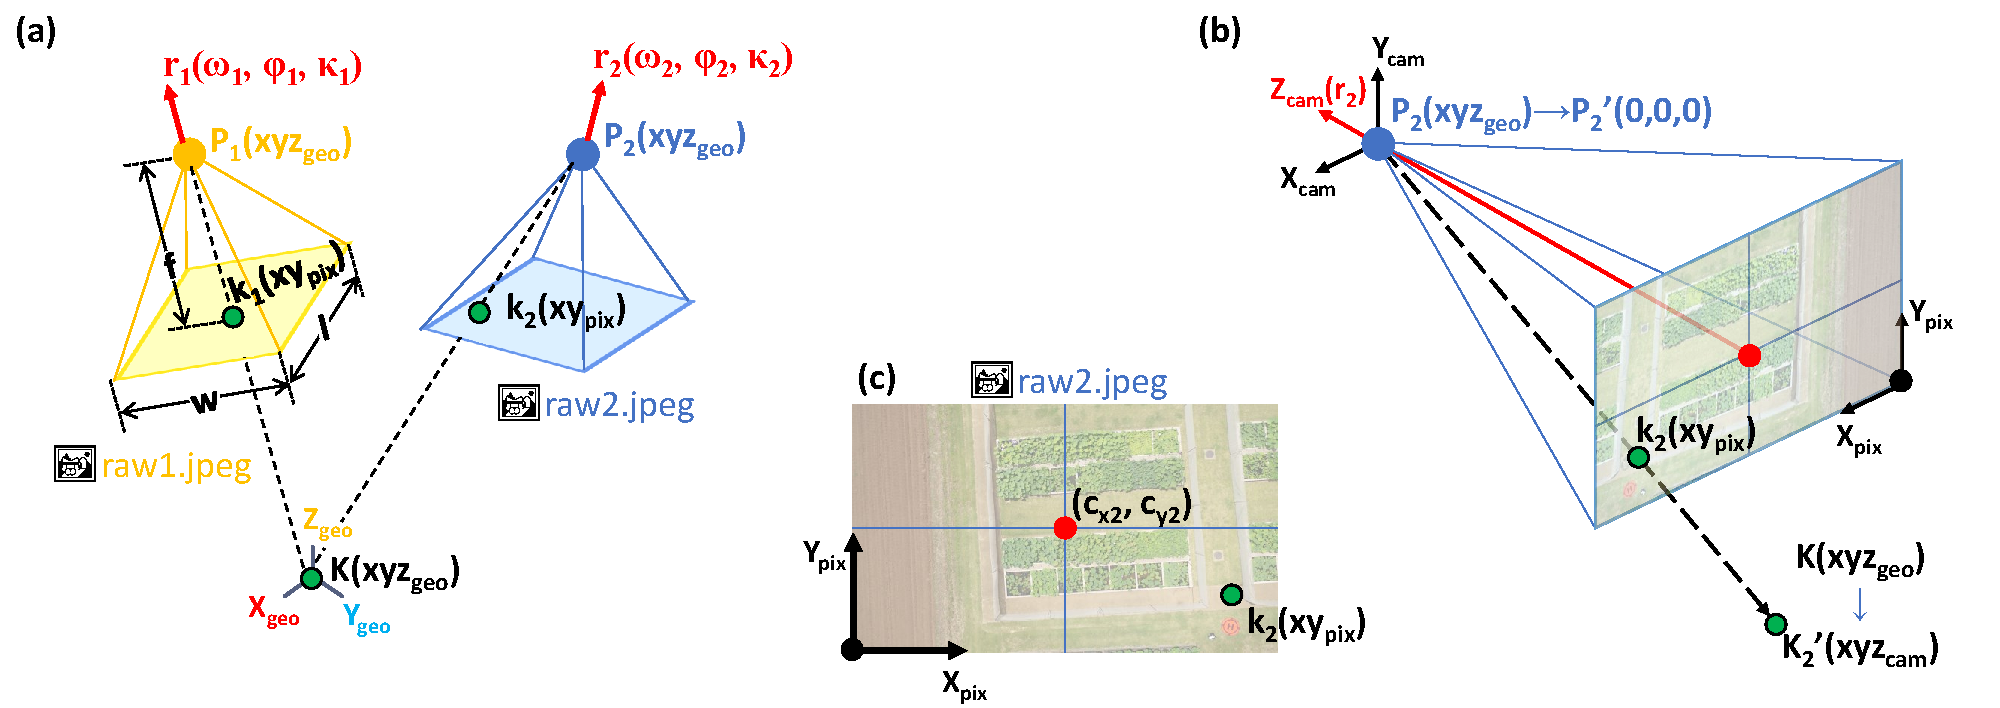
\includegraphics[width=0.95\linewidth]{figures/raw2raw.pdf}
    %\caption{tbc}
    \label{Apd:raw2raw}
  \end{figure}
  text text text

  \subsection*{Additional file 2 --- Sample additional file title}
  \begin{figure}[!h]
    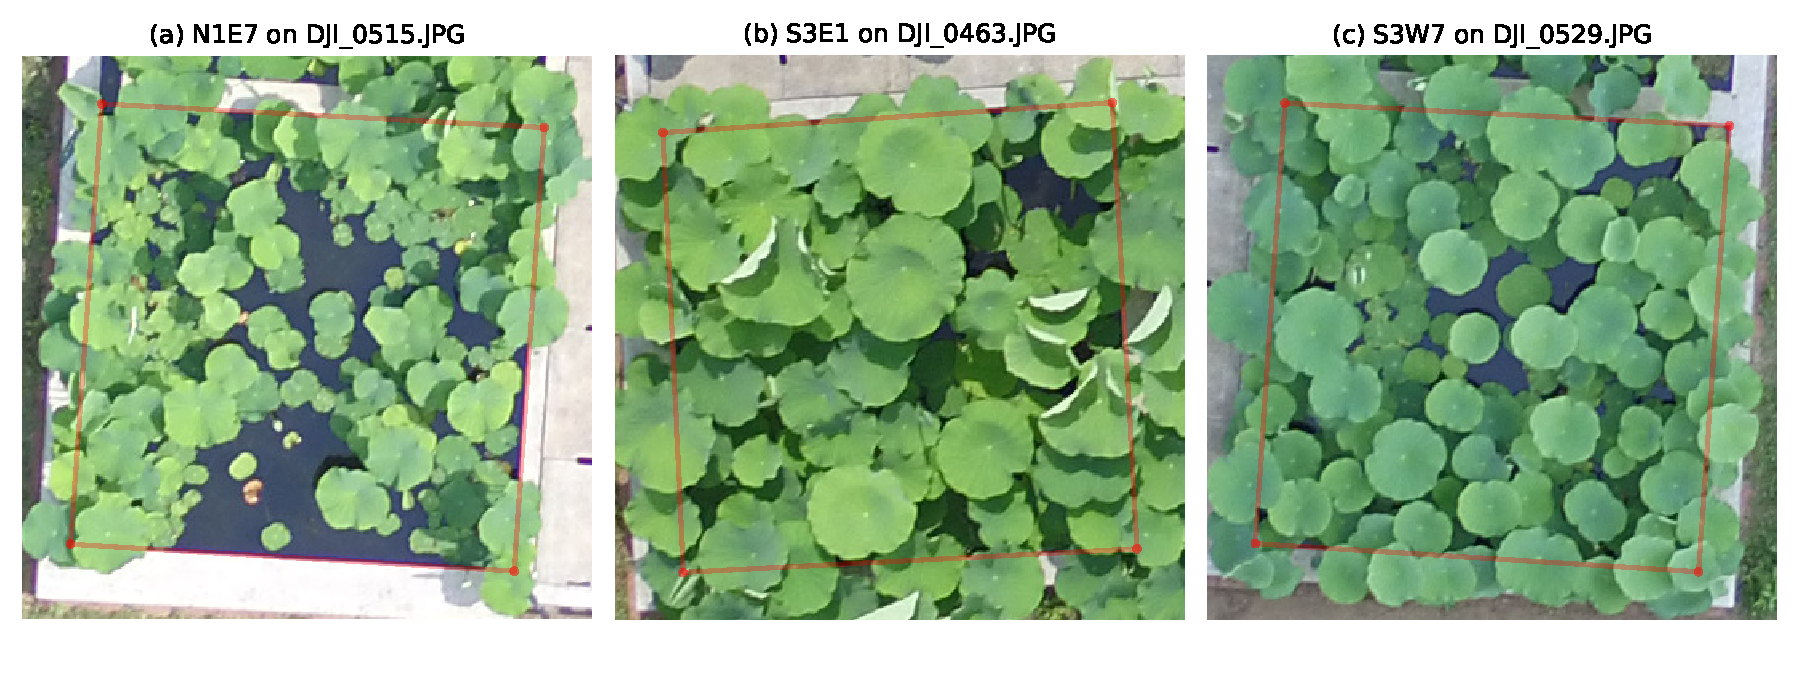
\includegraphics[width=0.95\linewidth]{figures/difficult_ground.pdf}
    %\caption{tbc}
    \label{Apd:diff}
  \end{figure}

  Text text text

  \subsection*{Additional file 3 --- Sample additional file title}
  \begin{figure}[!h]
    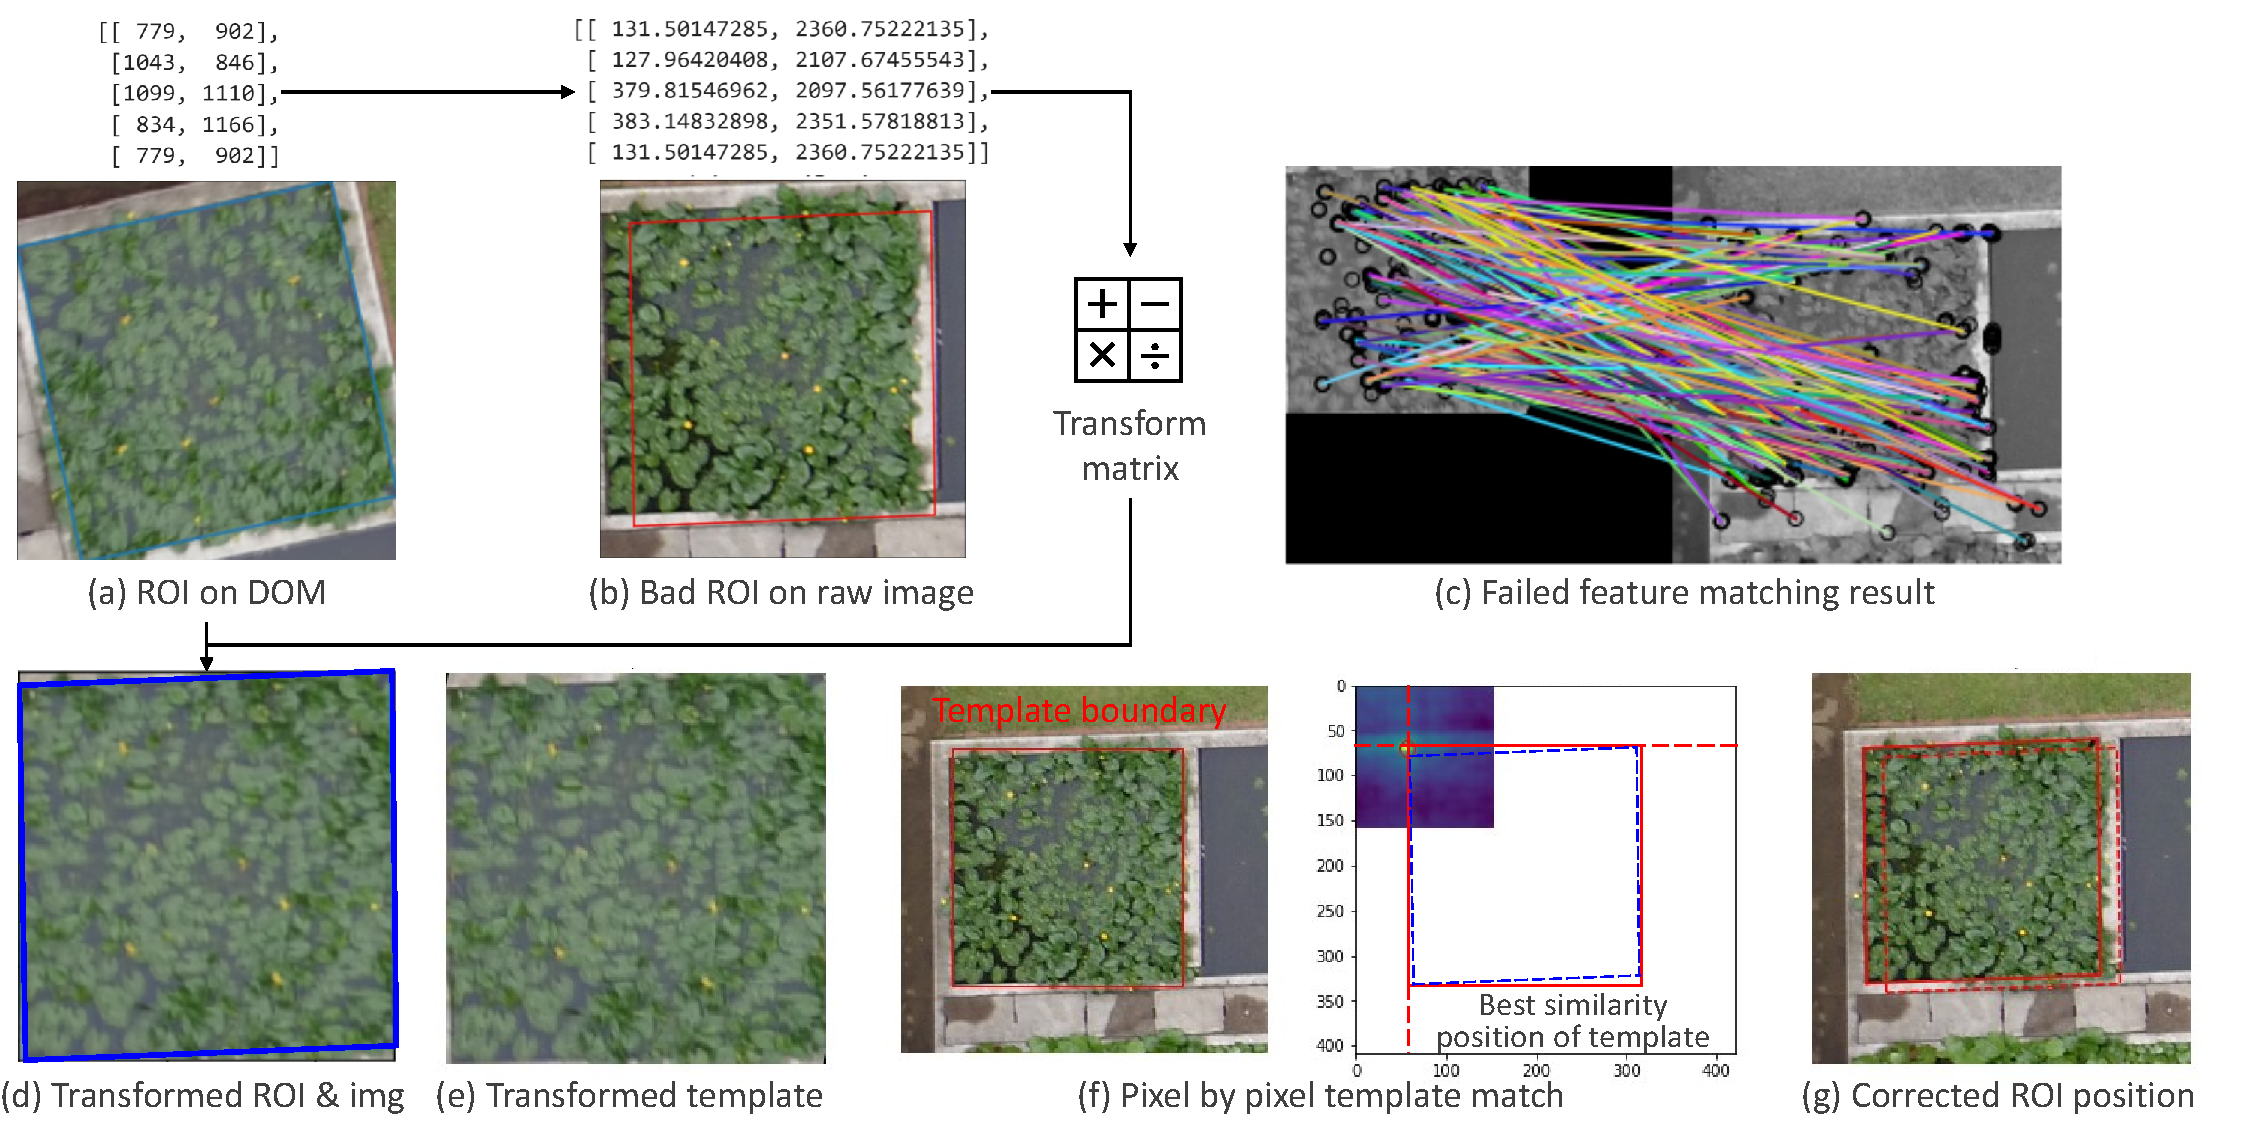
\includegraphics[width=0.95\linewidth]{figures/template_match.pdf}
    %\caption{tbc}
    \label{Apd:template}
  \end{figure}

  Text text text

\end{backmatter}

\end{document}